\documentclass[11pt]{standalone}

\usepackage{lmodern}    % font definition
\usepackage{amsmath}    % math fonts
\usepackage{amsthm}
\usepackage{amsfonts}
\usepackage{pgfplots}

\usepackage{pgfplots}
\usepackage{xcolor}
\usetikzlibrary{positioning,bayesnet}
\definecolor{brinkpink}{rgb}{0.98, 0.38, 0.5}
\definecolor{aogreen}{rgb}{0.0, 0.5, 0.0}
\usepackage{tikz}
\usetikzlibrary{decorations.pathmorphing} % noisy shapes
\usetikzlibrary{fit}                    % fitting shapes to coordinates
\usetikzlibrary{backgrounds}    % drawing the background after the foreground
\pgfplotsset{compat=newest}% <-- moves axis labels near ticklabels (respects tick label widths)

\begin{document}
  \pgfplotsset{every tick label/.append style={font=\small}}
  \pgfplotsset{every axis label/.append style={font=\small}}
  \pgfplotsset{
    every axis/.append style={%
      gray!30
    }
  }



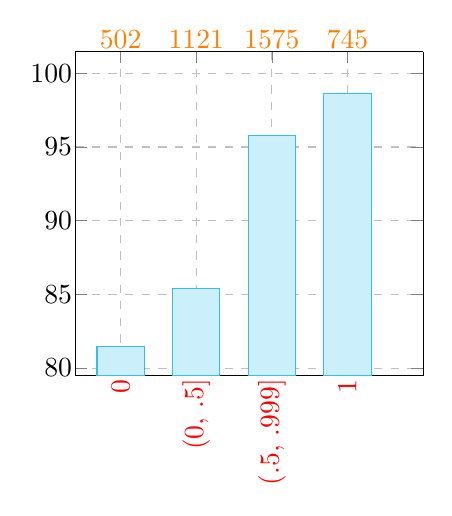
\begin{tikzpicture}
  \centering
  
  \begin{axis}[%ybar=1.0pt,
    axis x line*  = bottom,
    ybar stacked,
    height=5.699999999999999cm,
    width=6.0cm, % 12->9,  9->6.93,  8-> 6
    bar width=0.6cm,
    xmin=0.4,
    xmax=5,
    ymin=79.47,
    ymax=98.6,
    enlarge y limits={upper,value=0.15},
    legend style={at={(0.5,-0.25)},anchor=north,legend columns=-1,
    /tikz/every even column/.append style={column sep=0.2cm}},
    xticklabels={\textcolor{red}{0}, \textcolor{red}{(0, .5]}, \textcolor{red}{(.5, .999]}, \textcolor{red}{1}},
    xtick=data,
    xmajorgrids=true,
    ymajorgrids=true,
    zmajorgrids=true,
    grid style=dashed,
    xticklabel style={
        inner sep=1pt,
        rotate=90
    },
    yticklabel style={
        inner sep=1pt,
        black,
    },     
    ]
    
    \addplot [draw=cyan!80,fill=cyan!20] table[x=id,y=y]{
    id  y
    	1	81.47
	2	85.37
	3	95.77
	4	98.6
    };
  \end{axis}
  
  \begin{axis}[   
    axis x line* = top,
    axis y line  = none,
    ybar stacked,
    height=5.699999999999999cm,
    width=6.0cm, % 12->9,  9->6.93,  8-> 6
    bar width=0.6cm,
    xmin=0.4,
    xmax=5,
    ymin=79.47,
    ymax=98.6,
    enlarge y limits={upper,value=0.15},
    legend style={at={(0.5,-0.25)},anchor=north,legend columns=-1,
    /tikz/every even column/.append style={column sep=0.2cm}},
    xticklabels={\textcolor{orange}{502}, \textcolor{orange}{1121}, \textcolor{orange}{1575}, \textcolor{orange}{745}, },
    xtick=data,
    grid style=dashed,
    xticklabel style={
        inner sep=1pt,
    },
    ]
    \addplot [draw=cyan!80,fill=cyan!20] table[x=id,y=y]{
    id  y
    	1	81.47
	2	85.37
	3	95.77
	4	98.6
    };  
\end{axis}
  
  
\end{tikzpicture}

\end{document}


